% !TEX TS-program = pdflatex
% !TEX encoding = UTF-8 Unicode

% This is a simple template for a LaTeX document using the "article" class.
% See "book", "report", "letter" for other types of document.

\documentclass[11pt]{article} % use larger type; default would be 10pt

\usepackage[utf8]{inputenc} % set input encoding (not needed with XeLaTeX)
%\usepackage[table,xcdraw]{xcolor}
\usepackage{color}
%\usepackage{tabularray}
%%% Examples of Article customizations
% These packages are optional, depending whether you want the features they provide.
% See the LaTeX Companion or other references for full information.

%%% PAGE DIMENSIONS
\usepackage{geometry} % to change the page dimensions
\geometry{a4paper} % or letterpaper (US) or a5paper or....
% \geometry{margin=2in} % for example, change the margins to 2 inches all round
% \geometry{landscape} % set up the page for landscape
%   read geometry.pdf for detailed page layout information

\usepackage{graphicx} % support the \includegraphics command and options

% \usepackage[parfill]{parskip} % Activate to begin paragraphs with an empty line rather than an indent

%%% PACKAGES
\usepackage{booktabs} % for much better looking tables
\usepackage{array} % for better arrays (eg matrices) in maths
\usepackage{paralist} % very flexible & customisable lists (eg. enumerate/itemize, etc.)
\usepackage{verbatim} % adds environment for commenting out blocks of text & for better verbatim
\usepackage{subfig} % make it possible to include more than one captioned figure/table in a single float
\usepackage{hyperref}
\usepackage{float}
% These packages are all incorporated in the memoir class to one degree or another...

%%% HEADERS & FOOTERS
\usepackage{fancyhdr} % This should be set AFTER setting up the page geometry
\pagestyle{fancy} % options: empty , plain , fancy
\renewcommand{\headrulewidth}{0pt} % customise the layout...
\lhead{}\chead{}\rhead{}
\lfoot{}\cfoot{\thepage}\rfoot{}

%%% SECTION TITLE APPEARANCE
\usepackage{sectsty}
\allsectionsfont{\sffamily\mdseries\upshape} % (See the fntguide.pdf for font help)
% (This matches ConTeXt defaults)

%%% ToC (table of contents) APPEARANCE
\usepackage[nottoc,notlof,notlot]{tocbibind} % Put the bibliography in the ToC
\usepackage[titles,subfigure]{tocloft} % Alter the style of the Table of Contents
\renewcommand{\cftsecfont}{\rmfamily\mdseries\upshape}
\renewcommand{\cftsecpagefont}{\rmfamily\mdseries\upshape} % No bold!

%%% END Article customizations

%%% The "real" document content comes below...

\title{Microscopy data analysis practical - smFISH}
\author{Philipp Savakis, Evelina Tutucci}
%\date{} % Activate to display a given date or no date (if empty),
         % otherwise the current date is printed 

\begin{document}
\maketitle

\section{Overview}
In this practical, you will explore and analyse microscopy image data from a single molecule fluorescence {\it in situ} hybridisation (smFISH) experiment on single cells of {\it Saccharomyces cerevisiae}. This type of experiment allows the visualisation of individual mRNA molecules. 
You are handed fluorescence data from one location of a microscopy sample. 
The data consists of of three z-stacks, corresponding to the following channels:
\begin{itemize}
\item DAPI (bulk staining of nucleic acids - useful to find the location of the nucleus)
\item CY3 (visualises a specific mRNA - which one it is, you need to infer from the data) 
\item CY5 (visualises another specific mRNA - which one it is, you need to infer from the data)
\end{itemize}

\section{Setting up}
\subsection{required software and data}
\begin{itemize}
\item anaconda (install from \href{https://anaconda.com}{website}). You can install pycharm and/or spyder, but neither are required for this practical. 
\item image data folder from canvas (find the zip file pertaining to your group, download and unzip)
\end{itemize}

\subsubsection{setting up virtual environment for napari}
The software that you will be mainly interacting with is napari, a python based image viewer. 
For a clean setup, we will create a new python virtual environment. 
A virtual environment ensures that 
\begin{itemize}
\item we use an appropriate python version
\item all the dependencies (i.e. required software packages) are there
\item the dependencies for this project do not interfere with other software on your machine
\end{itemize}

We will delegate the work of creating/organising the virtual environment to anaconda. 

\subsubsection{navigation to correct folder}
{\bf Under windows}, hit the windows key and type anaconda. You should see 
\begin{verbatim} anaconda prompt \end{verbatim} 
as a choice. Open anaconda prompt. 

You should see a command line interface that looks something like:

\begin{verbatim} (base) C:\Users\YourUserName> _ \end{verbatim}


Use the command line to navigate to the unzipped data folder you downloaded from canvas. 
There, navigate to the {\it biophotonics} folder. 
type \begin{verbatim} dir \end{verbatim}
to explore the directory's contents.
You should find a file named \begin{verbatim} requirements.txt \end{verbatim}.

{\bf On mac}, navigate to the biophotonics folder in the group folder you downloaded from canvas. Right-click on the folder and select {\it open in new terminal window}.
You should see a command line interface that looks something like:

\begin{verbatim} (base) User@user: ~/whereever/you/donwloaded/the/folder/to/biophotonics$ _ \end{verbatim}

\subsubsection{creation of environment}
The {\it (base)} in your command line interface tells you that you are in the base environment - we have not created a custom environment yet. 
Now, create a new environment by typing the following:
\begin{verbatim} conda create -n biophotonics python=3.9 -y \end{verbatim}
This tells anaconda to create a new environment, which is named {\it biophotonics} and which will be set up using python version 3.9.
We include the -y flag to confirm installation of the libraries that anaconda will download. You can leave this out for fuller control, but then will have to manually confirm installations.

After the environment is created, we need to activate it. Type:
\begin{verbatim} conda activate biophotonics \end{verbatim}
On, windows, your command line should now show 
\begin{verbatim} (biophotonics) C:\The\location\of\your\group\folder> _ \end{verbatim}
 
On mac, you should see:
\begin{verbatim} (biophotonics) User@user: ~/whereever/you/donwloaded/the/folder/to/biophotonics$ _ \end{verbatim}

We will now make use of {\it pip} for installation of most packages. Convince yourself that the folder you have navigated to contains a file named requirements.txt. Now, type
\begin{verbatim} pip install -r requirements.txt \end{verbatim}
This should download a bunch of python libraries. After all is done, install the napari viewer, by typing:

\begin{verbatim} pip install napari[all] \end{verbatim}
 
 On mac, type
\begin{verbatim} python -m pip install ''napari[all]'' \end{verbatim}
  
To install the napari plugin for this course, type:
 
\begin{verbatim} pip install -e . \end{verbatim}
 
Then, open napari, by typing:
 
\begin{verbatim} napari \end{verbatim}
 
 If all is well, you should be looking at this window:
 
 \begin{figure}[H]
 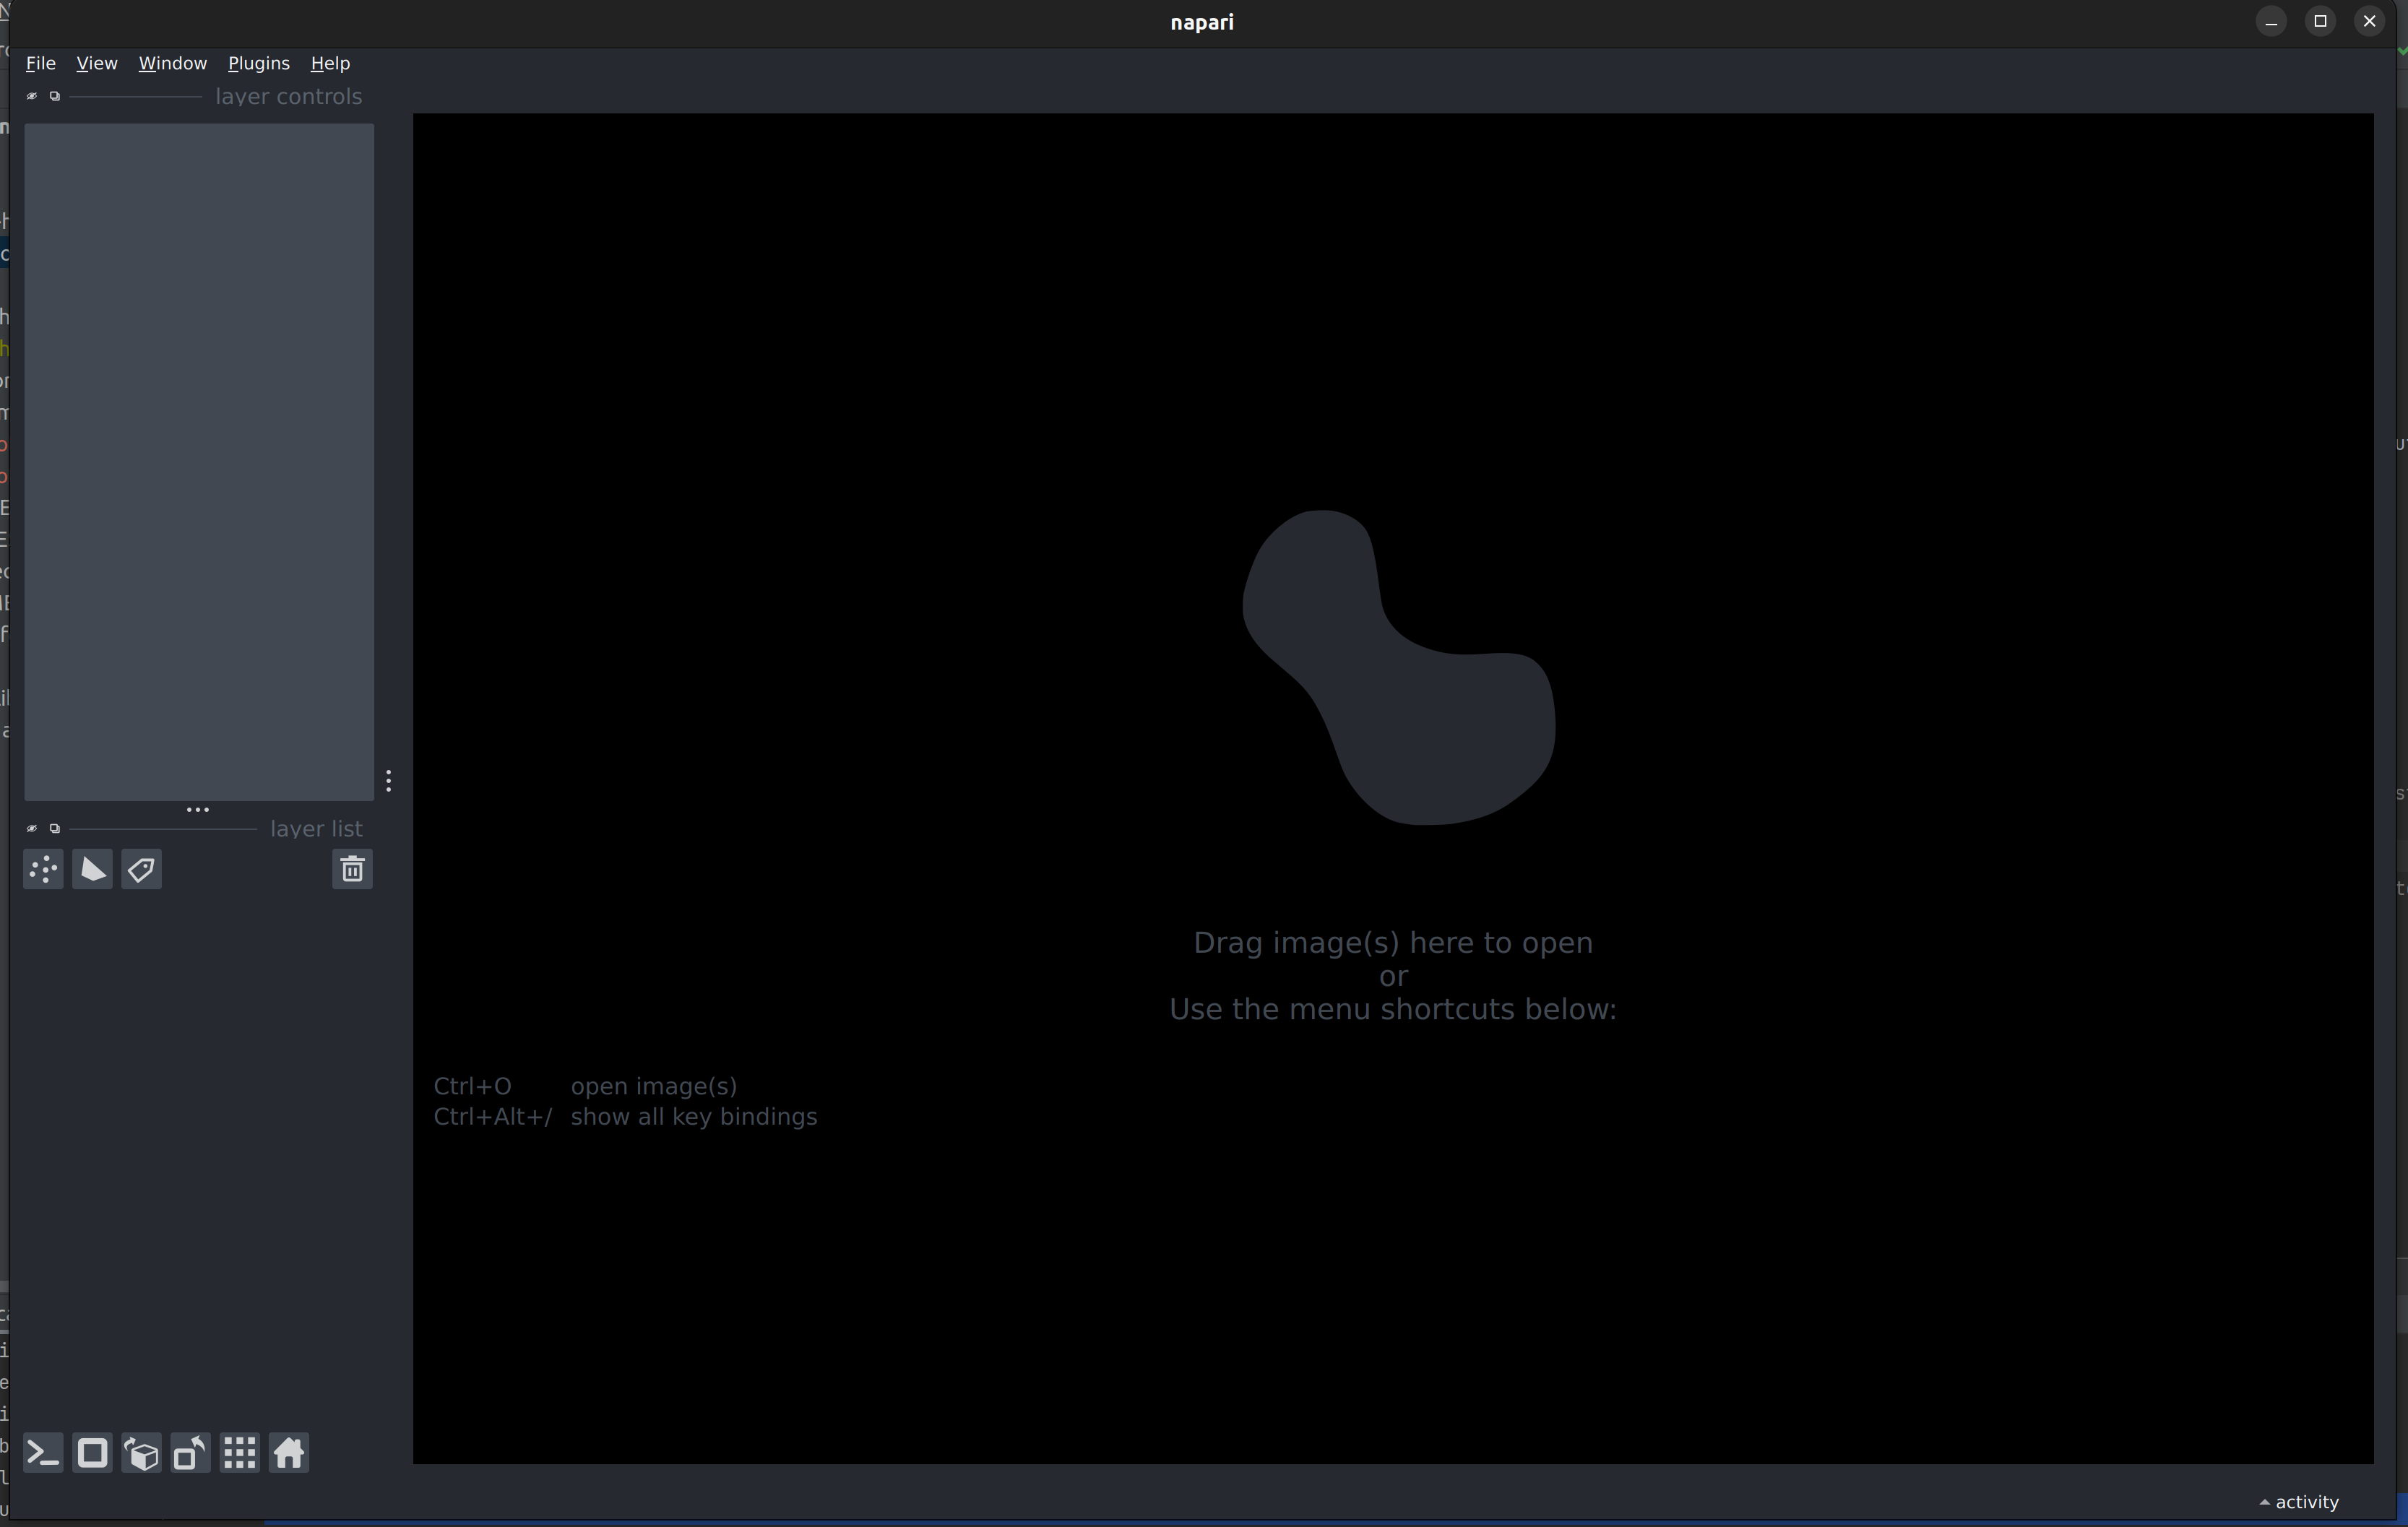
\includegraphics[width=14cm]{images/napari_viewer_1.png}
 \caption{napari user interface}
 \end{figure}
 
\section{data exploration with napari}
First, let's look at the data that was provided to you. 
Open the images by dragging them into the napari viewer. 
each .tif file in your /data/ folder has the following dimension: 41 x 2304 x 2304.
This means that each image consists of 41 images, with height and with of 2304 pixels each:
 
 % z-stack picture. 

You can visualise different z-layers through the slider at the bottom of the image. 

By default, napari makes no distinction between distances in the x,y,z direction. 
Most microscopes, however, have lower resolution in z than they do in x/y. 
This means that two pixels in z direction are further apart than two pixels in x/y direction.  

To tell napari that this is the case, we need to adjust layer scaling. We can do this by pressing the \begin{verbatim} >_ \end{verbatim}
button on the bottom left of the napari interface. 

This should open a console window. In there, type:

\begin{verbatim} viewer.layers[0].scale = [3, 1, 1] \end{verbatim}
\begin{verbatim} viewer.layers[1].scale = [3, 1, 1] \end{verbatim}
\begin{verbatim} viewer.layers[2].scale = [3, 1, 1] \end{verbatim}


Napari has powerful 3D visualisation functionality, which will allow us to explore the data in 3D. Press the square button next to the console button (or use the shortcut ctrl+y) in the napari interface. Now, the image should be transformed into a 3D image. 
Use your mouse to move around in the image. Use the menu to the left to manipulate colour representations and transparency/opactiy of the data. 
Can you create a 3D-overlay, which shows the mRNA spots and the nuclei? Take a screenshot for your report. 

When you are done exploring the data, restore the uniform scaling by typing:

\begin{verbatim} viewer.layers[0].scale = [1, 1, 1] \end{verbatim}
\begin{verbatim} viewer.layers[1].scale = [1, 1, 1] \end{verbatim}
\begin{verbatim} viewer.layers[2].scale = [1, 1, 1] \end{verbatim}

into the napari console. Exit 3D visualisation mode through ctrl+y

\section{image segmentation with napari}
In this practical, we want to say something about the number of transcripts in individual cells. To do this, we need to find individual cells first. 
To find them, we could label each individual cell by hand, but if we want to finish this practical today, we can use something slightly less labour-intensive:
\begin{itemize}
\item Find the {\it Plugins} menu item at the top of the napari user interface. 
\item Open the biophotonics/Random forest plugin.
\end{itemize}

Ensure that you are in 2D view mode. 
For computational reasons, we need to restrict cell segmentation to a single 2304 by 2304 image. 
We can generate this image from the z-stack, by generating a max projection. 
We will use the DAPI channel for segmentation.
So, 
\begin{itemize}
\item select the DAPI layer
\item adjust the z-layers you want to combine ({\it z level start/finish}) 
\item create the max projection with the {\it max projection} button.
\end{itemize}

This should create the following layers:
 
\begin{itemize}
\item \begin{verbatim}Labels \end{verbatim}
\item \begin{verbatim}FISH_DAPI max proj \end{verbatim}   
\end{itemize}

Now, 

\begin{itemize}
\item Select \begin{verbatim}Labels \end{verbatim}
\item Familiarise yourself with the interface on the left. 
\item use the drawing tools to label a part of the image. 
\item for background use colour 1 (brown in the default colouring)
\item for cell interior (nucleus and surroundings) use colour 2 (light blue in the default colouring)  
\item for the border between cell and background use colour 3 (purple in the default colouring)
\end{itemize}

\begin{figure}[H]
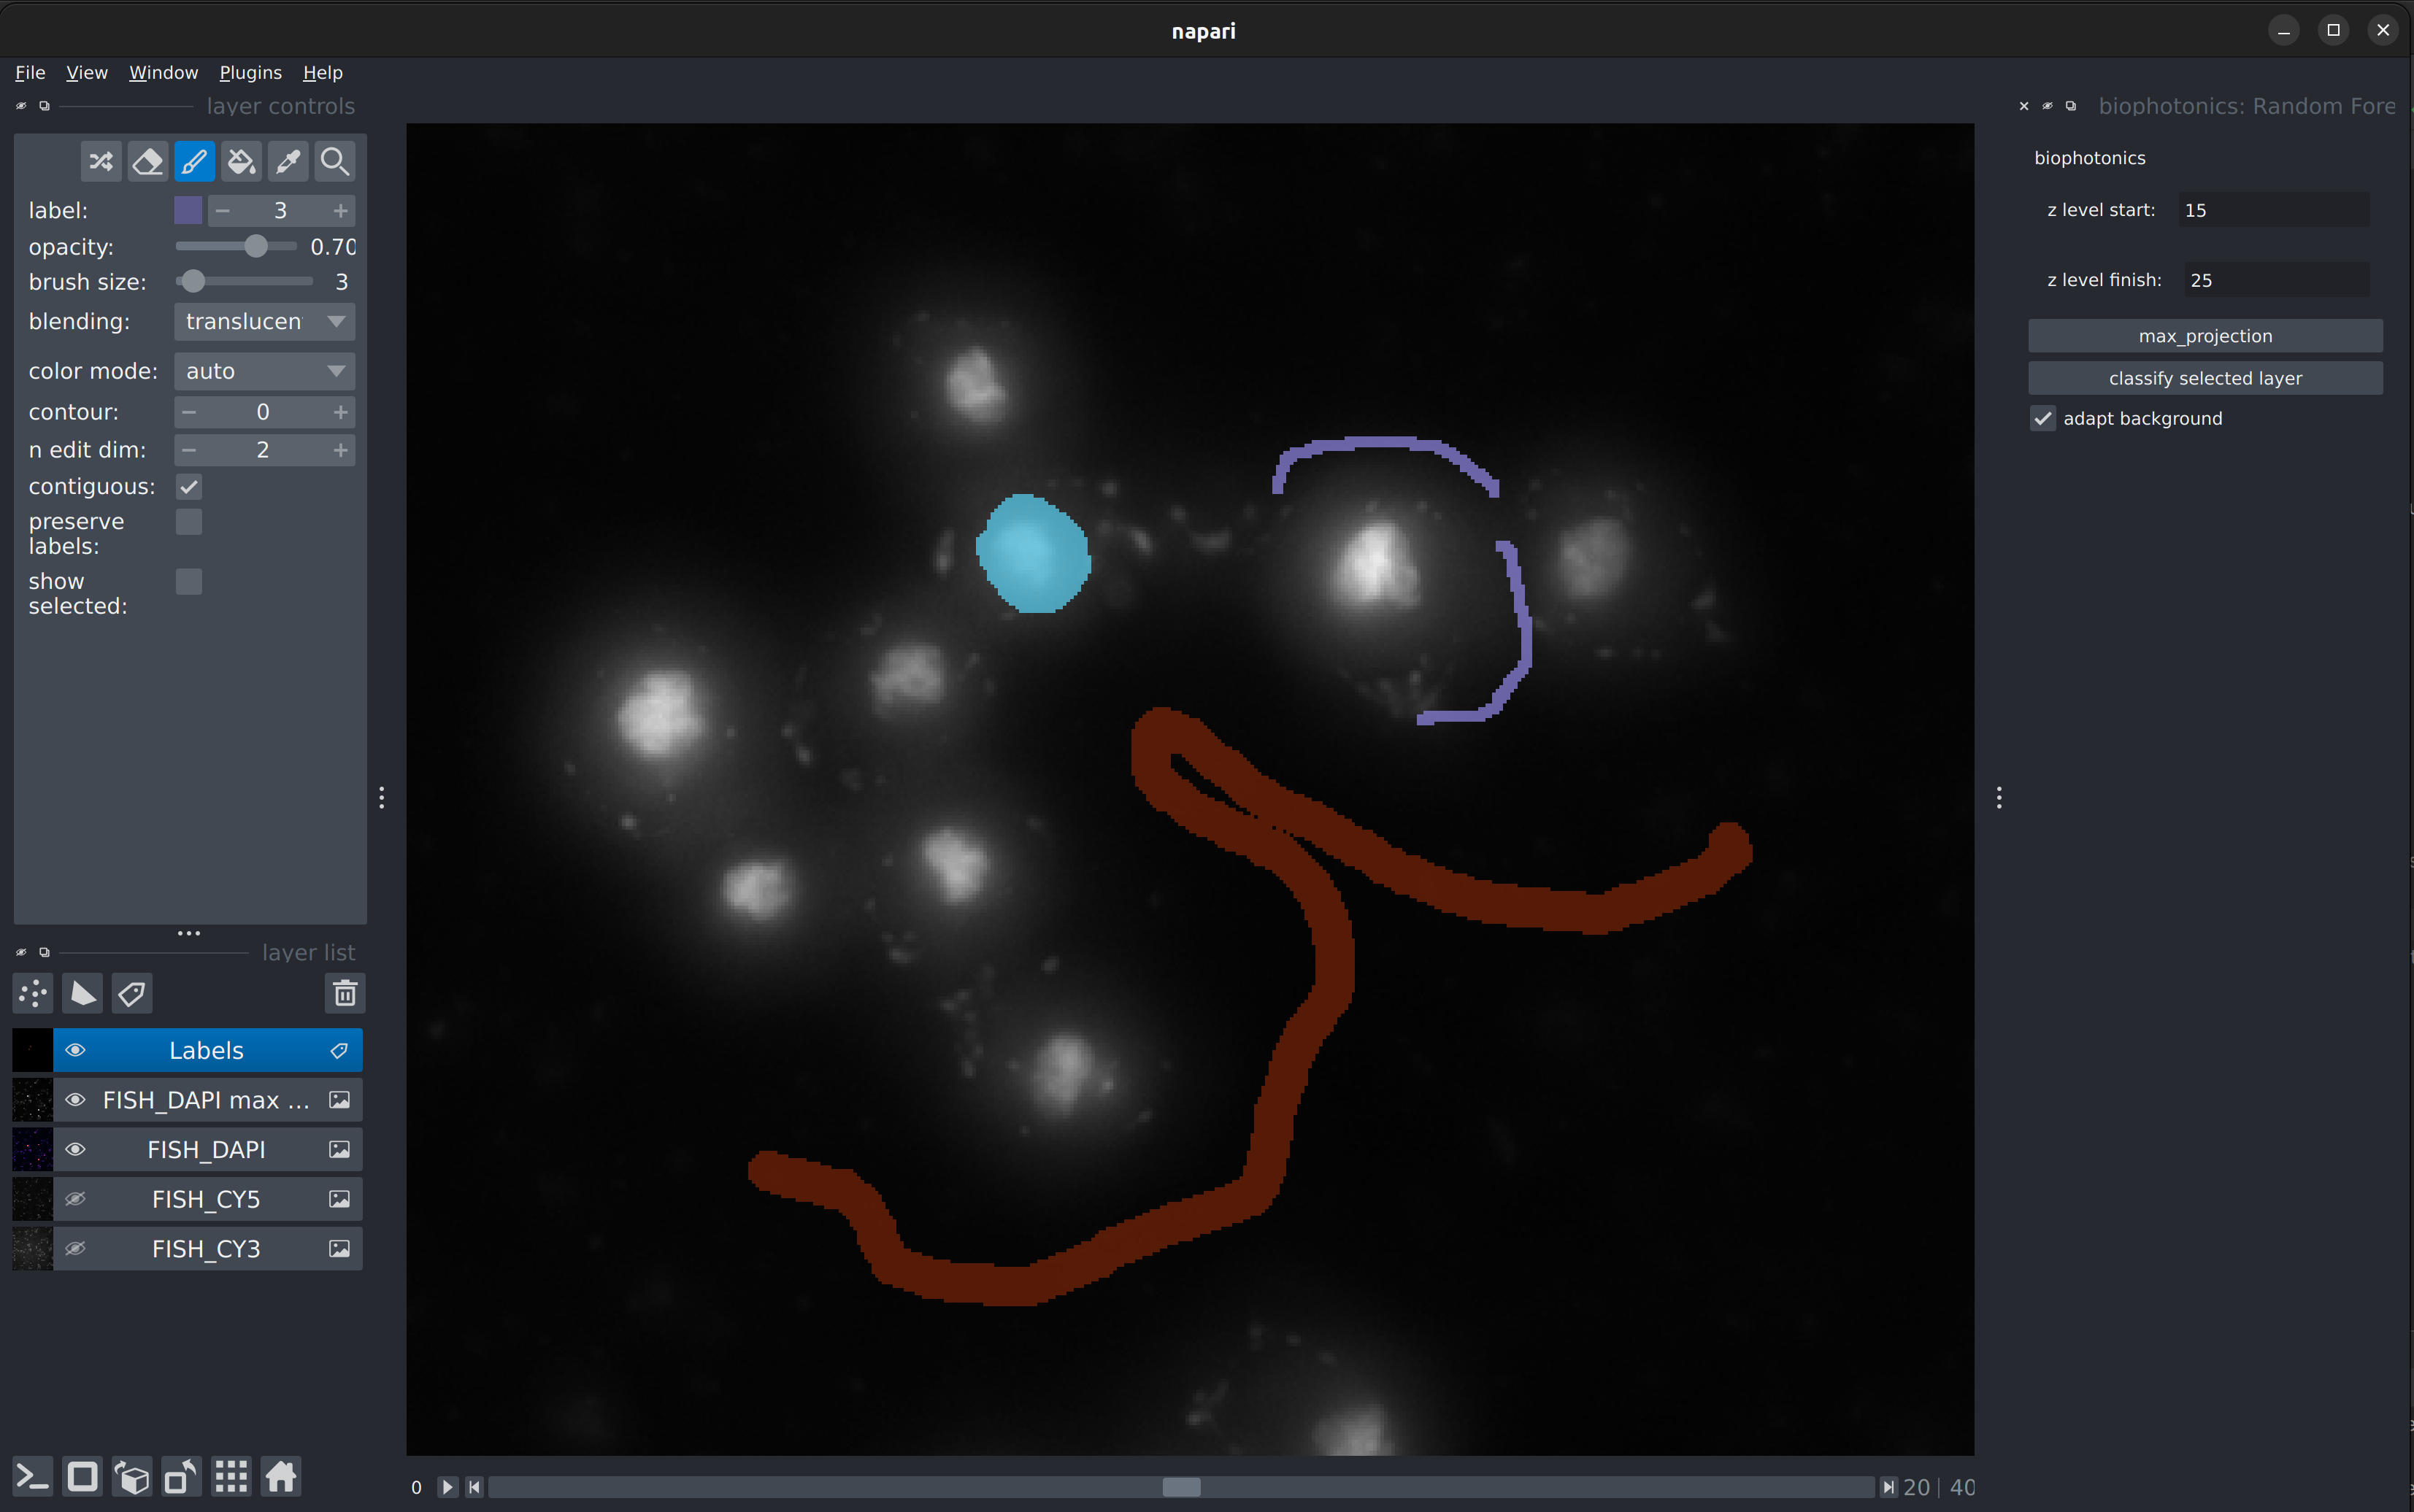
\includegraphics[width=14cm]{images/napari_viewer_6.png}
\caption{interactive generation of training examples for random forest algorithm}
\end{figure}

Make sure that you use exactly these colors, or the underlying segmentation routine will do funny things.
Once you are happy with your artwork
\begin{itemize}
\item select \begin{verbatim}FISH_DAPI max proj \end{verbatim}   
\item hit the button \begin{verbatim}classify selected layer\end{verbatim} 
\end{itemize}

This creates a new layer named \begin{verbatim} segmentation probabilites \end{verbatim}
This layer represents the random forest algorithm's belief that a given pixel in the image corresponds to a given class (background, cell interior, or border between cell and background).

Given this belief landscape, we need to now find regions in the image that belong to the same object. 
We will use the watershed algorithm to achieve this. 
The watershed algorithm needs seedpoints, which we can generate from the DAPI channel.
The rationale is that high fluorescence in the DAPI channel corresponds to a nucleus, and nuclei are typically at the centroid of a cell.


\begin{itemize}
\item Find the {\it Plugins} menu item at the top of the napari user interface. 
\item Open the biophotonics/watershed plugin.
\item select the FISH\_DAPI layer.
\item adjust the intensity/distance parameters and press {\it find nuclei}
\item remove superfluous layers (in case you had to use {\it find nuclei} more than once)
\item check the nuclei layer you generated and add/remove points as needed
\item select the {\it segmentation probabilities} layer
\item click the {\it watershed} button
\item this creates a {\it segmentation} layer. 
\item use the drawing tools to adjust cells as needed. 
\item save the segmentation image to disk (button on the right)
\end{itemize}

Saving the segmentation generates two files, one .tif file which holds the actual segmentation, and a .pkl file, which holds information about all the unique cell labels. We need this information later to indentify cells that are in the experiment but that have no 
mRNA counts. 

\section{Finding individual mRNAs}
Normally, we would take the 3D data in all its glory and perform preprocessing and 3D gaussian fitting to capture point light sources (corresponding to single mRNAs) as precisely as possible. 
This is unfortunately beyond the capabilty of most laptops.
Therefore, we have implemented a 2D spot finder for this practical.
\begin{itemize}
\item Find the {\it Plugins} menu item at the top of the napari user interface. 
\item Open the biophotonics/ spot finder plugin.
\item select the FISH\_CY5 layer and create a max projection
\item discard the Labels layer that was created here
\end{itemize}

Now, to make individual spots more prominent, we will use a trick, in which the image is copied, and gaussian filters with different standard deviations are run over the indivudal copies. 
Then the difference between the images is computed (difference of gaussian, DoG). 

You can adjust the gaussian filter through the sigma parameters, and then hit {\it compute difference of gaussian}. 
Play around with the values and inspect the resulting images. 

Now, after having transformed the image with DoG, look at pixel intensities. 

\begin{itemize}
\item Select the {\it difference of gaussian} layer 
\item move your cursor over the image
\item at the bottom left of the napari user interface, you should see numbers corresponding to the xy position, and to the intensity at a given point
\item find, which values are typical for background pixels
\item do the same for spot pixels
\item find a threshold value inbetween two separate spots from background
\item hit the threshold button
\item adjust the newly created coords layer as needed, e.g.:
\end{itemize}

\begin{figure}[H]
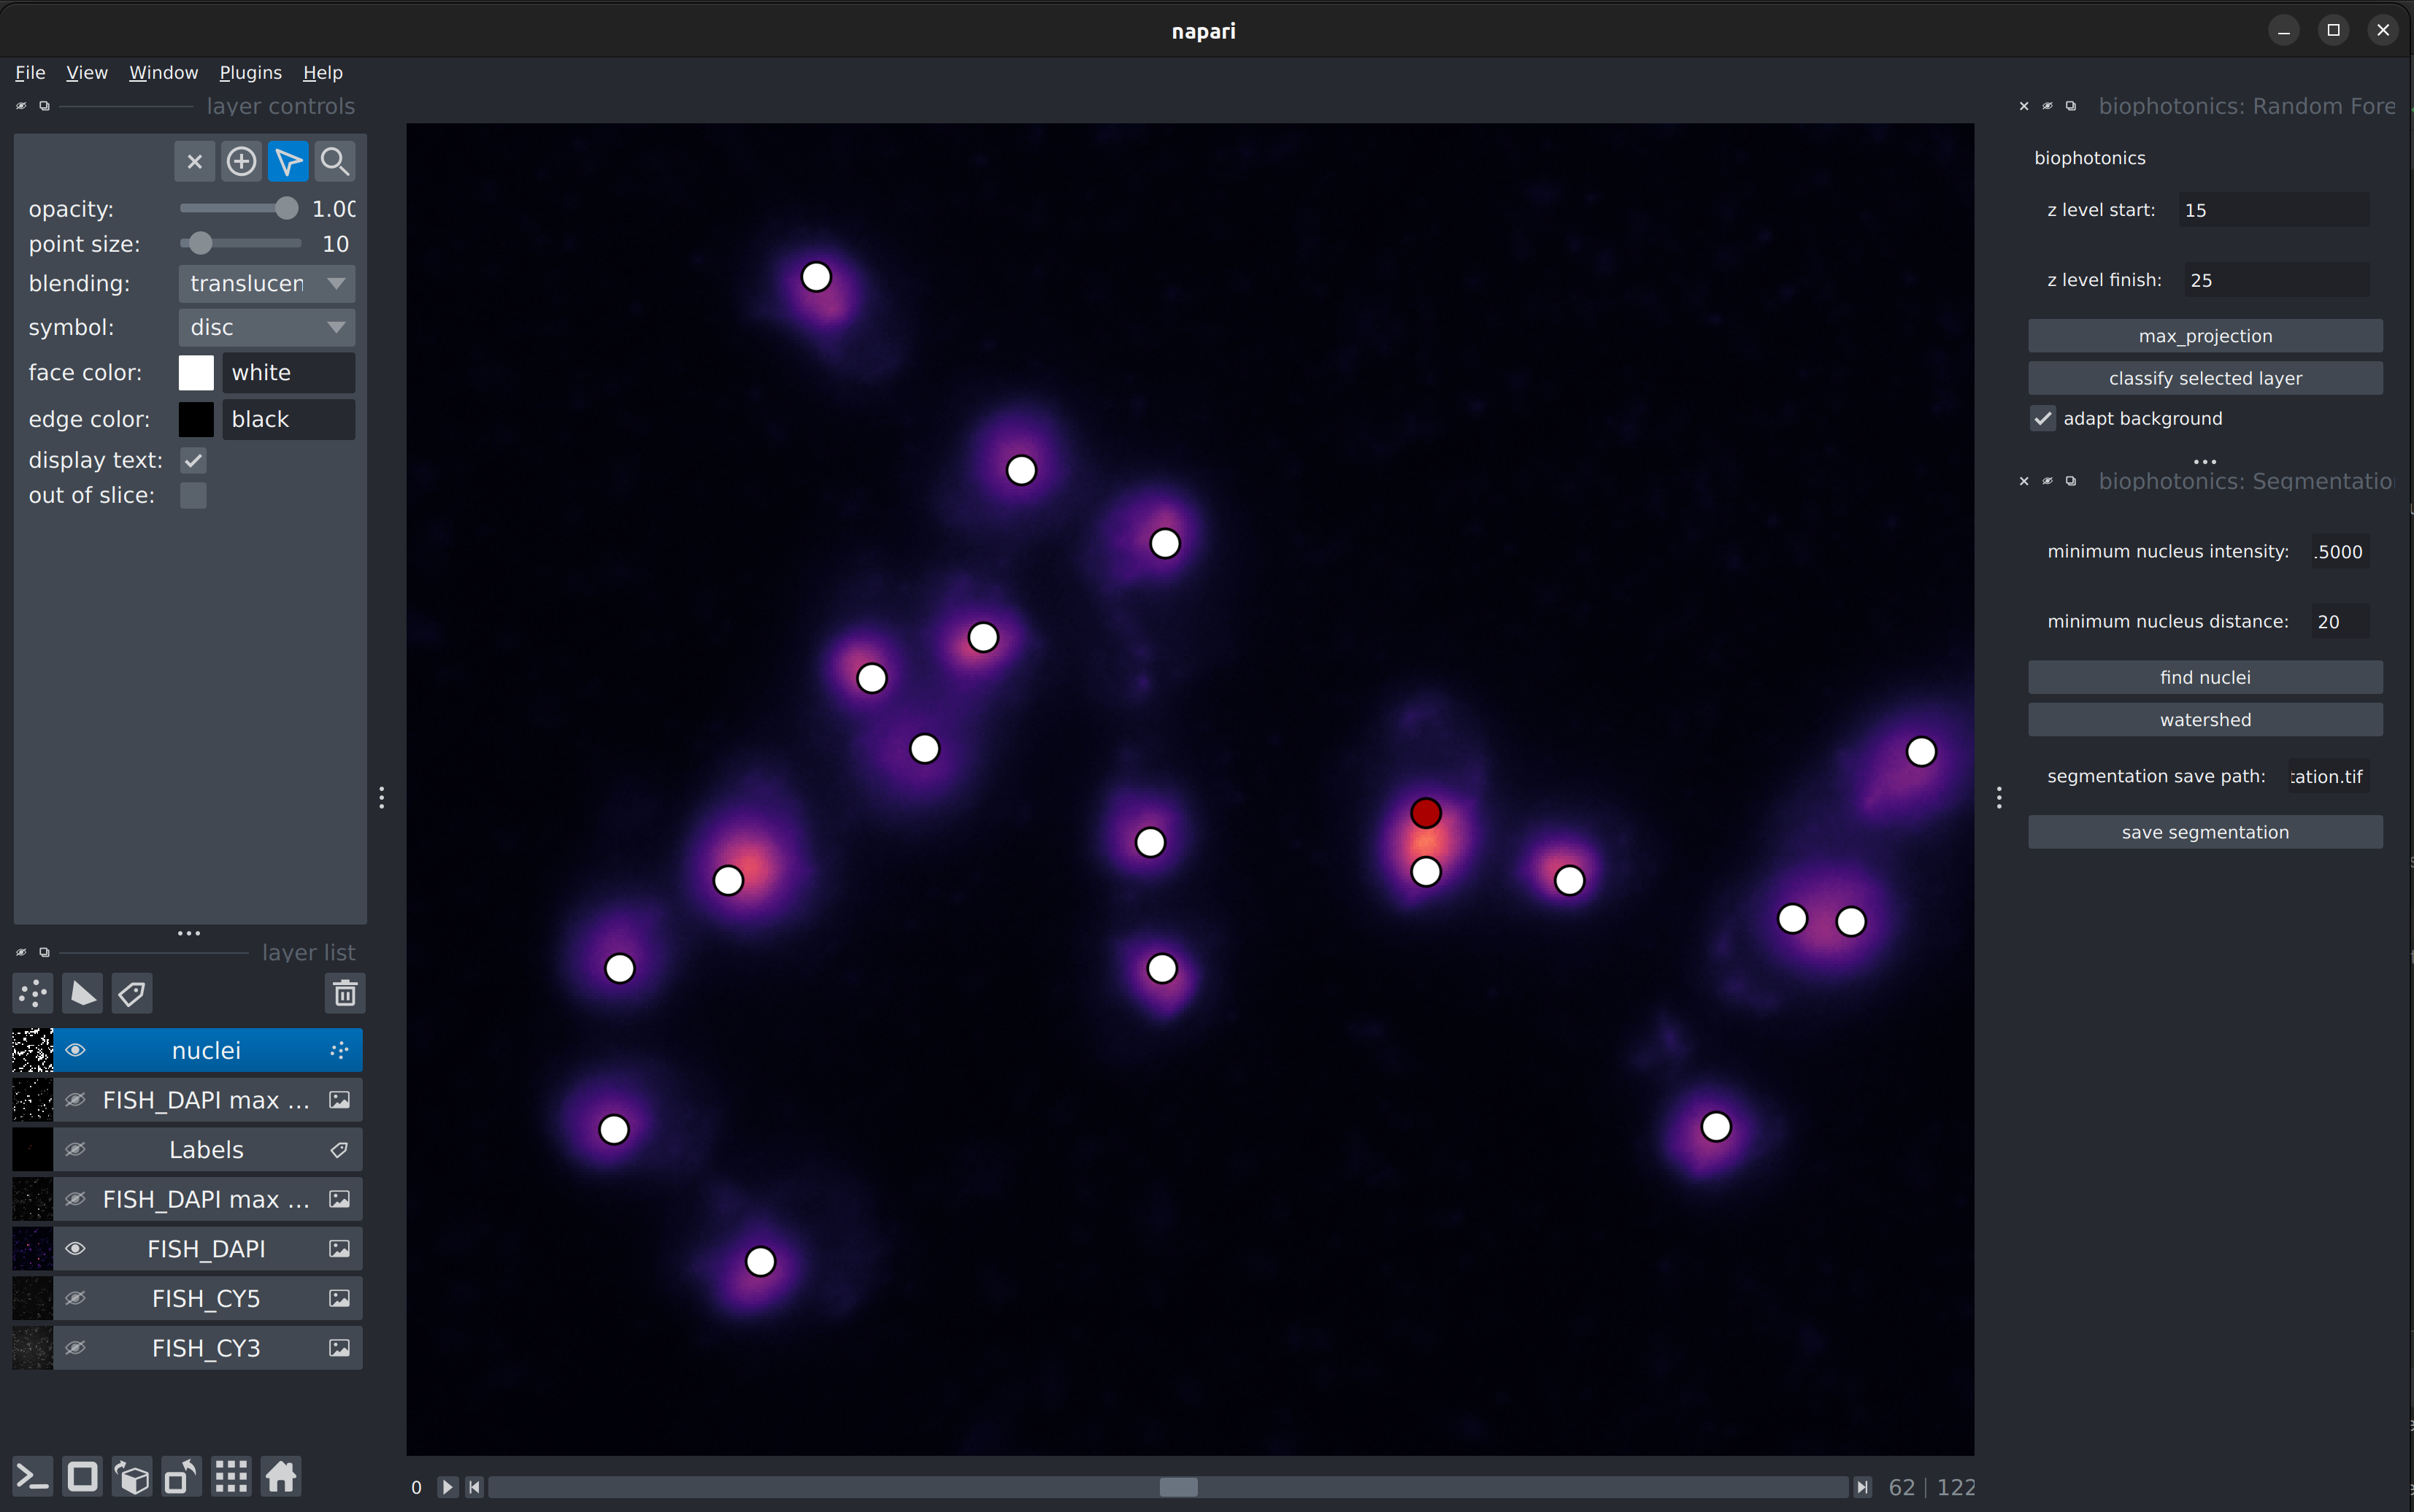
\includegraphics[width=14cm]{images/napari_viewer_7.png}
\caption{nuclei coordinates after nuclear detection. Sometimes two spots are identified. Adjust these as needed.}
\end{figure}

\begin{itemize}
\item now, ensure that all the right layers are selected: spot-intensity layer should be your CY-max projection, and spot position layer is the layer that you created during thresholding. 
\item save the spots to a pkl file using the {\it save spot information} button
\item repeat this section for the other channel, FISH\_CY3
\end{itemize}

\section{data processing}
You should now be the proud creator of two .pkl files. These files are in a storage format that allows data/object exchange between different python instances. Your file system likely will not know what to do with them. 

To look at the content of your files, 
\begin{itemize}
\item open a new instance of anaconda prompt (windows) or terminal (mac/linux)
\item no need to activate the napari environment here - the base environment should have all we need 
\item navigate to the folder {\it notebooks} in the biophotonics folder you downloaded from canvas
\item type \begin{verbatim} jupyter notebook \end{verbatim}
\item open \begin{verbatim} data_plotting.ipynb \end{verbatim}
\item follow the steps laid out in the notebook
\end{itemize}

\section{Finally}
Find out which mRNAs were fished for in your group.

\section{Report guidelines}
The report should be divided into four sections:

\begin{enumerate}
\item Aim of the study
\item Methods
\item Results
\item Conclusions
\end{enumerate}

You should 
\begin{itemize}
\item describe the biological question and the imaging methods employed to create the datasets that you received. 
\item describe segmentation and spot detection (show pictures of the results)
\item discuss problems and limitations of the approach
\item add histograms for cell counts per cell and for mRNAs per transcription site and any further analysis that you think is important for this practical. 
\item discuss results and define gene expression mode of the genes you were assigned. 
\end{itemize}

%\definecolor{OxfordBlue}{rgb}{0.176,0.231,0.27}
\begin{table}
%\centering
\begin{tabular}{|l | l| l|}
\hline
\textbf{Criteria}                                                                                                                                                                                                                                                & \textbf{Ratings}                                                                    & \textbf{Pts} \\
\hline
\hline
This criterion is linked & This area will be used by the assessor&\\
 to a learning outcome & to leave comments related to this criterion& \\
\hline
{\bf Structure and clarity of the narrative} &  & 30   \\
The report contains clearly defined parts:&&\\
&&\\
abstract, &&\\ 
introduction,&& \\ 
methods, &&\\
results, &&\\
discussion, &&\\
references &&\\
&&\\
All these parts have appropriate content&&\\
The storyline makes sense, &&\\
there is logic in the transitions&&\\ 
&&\\
Report is complete and not excessively long&&\\
\hline
{\bf Correct representation of facts} & & 20\\
The facts taken from the literature or &&\\
from your own knowledge are true&&\\
 Literature references are used&&\\
\hline
{\bf Data analysis and conclusions}& & 30\\
Data analysis is done properly&&\\
and obtained results are shown&&\\
You critically analyze obtained results &&\\
and draw logical conclusions&&\\
%{This criterion is linked to a learning outcome
\hline
{\bf Layout and figures }& & 10\\

The figures are well visible and explained, &&\\
and clearly illustrate your text&&\\
Proper use of &&\\
fonts, &&\\
margins,&&\\
 line spacings, etc &&\\
\hline
{\bf Grammar and spelling} & & 10\\
Minor mistakes and typos are not counted&&\\                                                                                                                                                          
\hline
\hline
&& 100\\
\hline
\end{tabular}
\end{table}

\end{document}
